\section{水流し試験}
本実験では流量計測にタービン流量計の他にオリフィス差圧とインジェクタ差圧を使用した。
差圧から流量を計測するために、各差圧の流量係数を確認する必要がある。
GHe供給圧をパラメータとし、水を30秒以上流し、噴出した水の総量から、水の流量を求めた。水の噴射の様子を図に示す。
\\
流量定数はベルヌーイの定理と連続の式から導出できる。
\begin{eqnarray}
P_{1} + \frac{1}{2} \rho_{1} u^2_{1} &=& P_{2} + \frac{1}{2} \rho_{2} u^2_{2}  \nonumber \\
u^2_{2} - u^2_{1} &=& \frac{2(P_{1}-P_{2})}{\rho} 
\label{eq:vel}
\end{eqnarray}
\begin{eqnarray}
u_{1}A_{1} &=& u_{2}A_{2}  \nonumber \\
u_{2} &=& u_{1}\frac{A_{1}}{A_{2}}
\label{eq:con}
\end{eqnarray}
\ref{eq:con}を\ref{eq:vel}に代入する。
\begin{eqnarray}
u_{2}=\frac{1}{\sqrt{1-(\frac{A_{2}}{A_{1}})^2}}\sqrt{\frac{2(P_{1}-P_{2})}{\rho}}
\label{eq:Velocity}
\end{eqnarray}
流量は$Q=u_{2}A_{2}$であるので、
\begin{eqnarray}
Q=u_{2}A_{2}=\frac{A_{2}}{\sqrt{1-(\frac{A_{2}}{A_{1}})^2}}\sqrt{\frac{2(P_{1}-P_{2})}{\rho}}
\label{eq:VFlux}
\end{eqnarray}
となり流量が求まる。ここで$CA=\frac{A_{2}}{\sqrt{1-(\frac{A_{2}}{A_{1}})^2}}$とすると、
\begin{eqnarray}
Q=CA\sqrt{\frac{2(P_{1}-P_{2})}{\rho}}
\label{eq:IdealFlux}
\end{eqnarray}
となる。$C$は流量係数で、$C=\frac{流量実測値}{流量計算値}$で求まる。$A$はオリフィス断面積である。
オリフィス断面積は$2.01 \times 10^{-6}mm$,インジェクタ断面積は$1.41 \times 10^{-6}mm$である。
本試験結果を表\ref{tab:Water}に示す。
\\
本試験でのインジェクタ及びオリフィスでの流量係数はそれぞれ$0.52$と$1.06$となった。
インジェクタの流量係数が設計時の想定流量係数$0.7$より小さくなった。
これはインジェクタ上流のマニホールド部の体積が小さく、流れの整流が十分ではなく、インジェクタ孔へ流れる流体の抵抗が大きくなったことが原因として考えられる。
\\
オリフィス流量係数は、$1$を超えている。計算上のオリフィス内径は$1.6mm$を用いているが、実際使用したものは$1.6mm$以上あるからと思われる。
\\
この試験により、実験上問題となる以上はないことが確認できた。

\begin{table}[htb]
\begin{center}
\caption{水流し試験結果}
\scriptsize
%\begin{tabular*}{200mm}{@{\extracolsep{\fill}}|c|c|c|c|c|c|c|c|c|c|} \hline
\begin{tabular}{|c|c|c|c|c|c|c|c|c|c|} \hline
No. & \shortstack{設定He\\圧力} & \shortstack{インジェクタ\\上流圧} & 流量 & \shortstack{インジェクタ\\差圧} & \shortstack{インジェクタ\\流量} & \shortstack{インジェクタ\\流量係数} & \shortstack{オリフィス\\差圧} & \shortstack{オリフィス\\理論流量} & \shortstack{オリフィス\\流量係数} \\ \cline{2-10}
 & MPaA & MPaA & L/s & MPa & L/s & - & MPa & L/s & - \\ \hline
1 & 0.6 & 0.55 & 0.021 & 0.45 & 0.042 & 0.51 & 0.058 & 0.022 & 0.99 \\ \hline
2 & 1.09 & 0.94 & 0.030 & 0.84 & 0.058 & 0.52 & 0.102 & 0.029 & 1.05 \\ \hline
3 & 1.61 & 1.40 & 0.037 & 1.30 & 0.072 & 0.51 & 0.149 & 0.035 & 1.06 \\ \hline
4 & 2.12 & 1.82 & 0.043 & 1.72 & 0.083 & 0.52 & 0.200 & 0.040 & 1.06 \\ \hline
5 & 3.10 & 2.68 & 0.053 & 2.58 & 0.102 & 0.52 & 0.300 & 0.049 & 1.07 \\ \hline
\end{tabular}
\label{tab:Water}
\end{center}
\end{table}

\begin{figure}[htb]
\centering
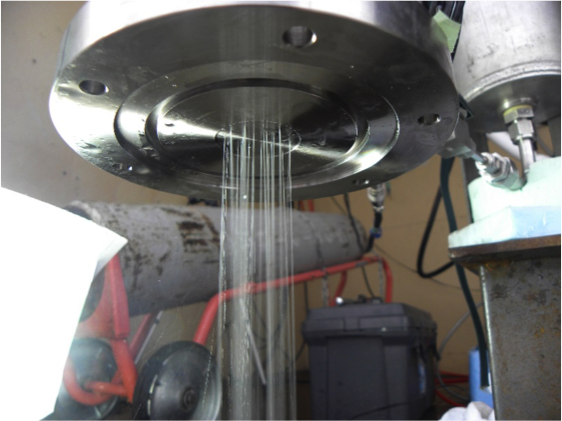
\includegraphics[width=13cm]{\FigAddTwo/Injector.png}
\caption{インジェクタ外観}
\label{fig:Injector}
\end{figure}
